\documentclass[a4paper]{article}

\usepackage{amssymb,mathrsfs,amsmath,amscd,amsthm}
\usepackage[mathcal]{euscript}
\usepackage{stmaryrd}
\usepackage[T1]{fontenc}
\usepackage[polish]{babel}
\usepackage{enumitem}
\usepackage{titling}
\usepackage{float}

%Image-related packages
\usepackage{graphicx}
\usepackage{subcaption}
\usepackage[utf8]{inputenc}
\usepackage[export]{adjustbox}
\usepackage{wrapfig}
%------------------------------

\setlength\parindent{0pt}

\title{Report}
\author{Marcin Mazur}

\begin{document}

\maketitle

\section{Loss}
As loss function I used \textit{BCE} and \textit{Focal loss}. As my predictions at the beginning,
were almost always blank or full, I added another parameter called \textit{round\_ratio} that
weights loss that was measured on masks that were discretized, in other words for final output
of the model (that is masks of 0 and 1, not the probabilities). The idea was to make model
predictions that can be better in practice and not just loss-wise. I had tested loss with both
\textit{BCE} and \textit{Focal} versions, \textit{BCE} turned out to be more stable, but \textit{Focal}
gave me better results, e.g. once I got $0.9$ iou, but unfortunately I couldnt reproduce that phenomenon.

\section{Optimization}
When it comes to optimizers I didn't see difference between \textit{Adam} and \textit{RMSprop}.
Best choice turned out to be starting with learing rate equal to $10^{-3}$ with warmup and train for the first
few epochs only non-backbone parameters. After that I was adding rest of the parameters, and starting again
with warmup, making newly added parameters' learing rate a little lower than the others. Throughout the whole process
I used scheduler for dropping on plateau.

\section{Lambda}
I tested various amounts of lambda, from $0$ to $0.5$. I could see that with bigger amounts, edges could
be really good, but whole mask wasnt necessarily better. I achieved best results for lambdas between $0.1$
and $0.2$. I think the thing that made the biggest change in training with edges was when I made my convs
take not one pixel of edge, but two (make edges a little wider). It made model training more stable,
the reason why I made the decision was the issue - how can model predict such in-continous states, with
mask moved just one pixel the value changes from max to min (1 to 0). Probably if I made it even wider
with more continous change it would show even better results.
\newpage
Here is a comparision of IOU for different lambdas smaller than $0.1$:
\begin{figure}[h]
    \centering
    \begin{subfigure}[b]{0.45\textwidth}
        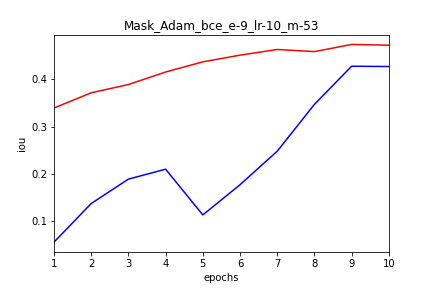
\includegraphics[width=\textwidth]{imgs/lambda/0/Mask_Adam_bce_e-9_lr-10_m-53_13_May_2022-22:17.png}
        \caption{Mask.}
    \end{subfigure}
    \hfill
    \begin{subfigure}[b]{0.45\textwidth}
        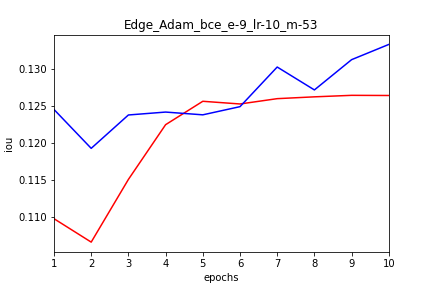
\includegraphics[width=\textwidth]{imgs/lambda/0/Edge_Adam_bce_e-9_lr-10_m-53_13_May_2022-22:17.png}
        \caption{Edge.}
    \end{subfigure}
    \caption{Lambda: 0}
\end{figure}

\begin{figure}[h]
    \centering
    \begin{subfigure}[b]{0.45\textwidth}
        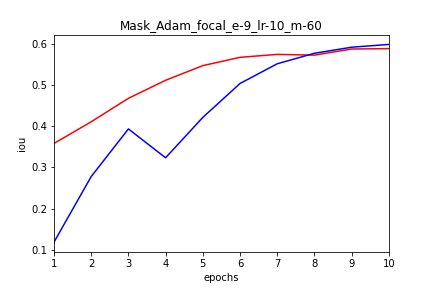
\includegraphics[width=\textwidth]{imgs/lambda/5/Mask_Adam_focal_e-9_lr-10_m-60_13_May_2022-22:32.png}
        \caption{Mask.}
    \end{subfigure}
    \hfill
    \begin{subfigure}[b]{0.45\textwidth}
        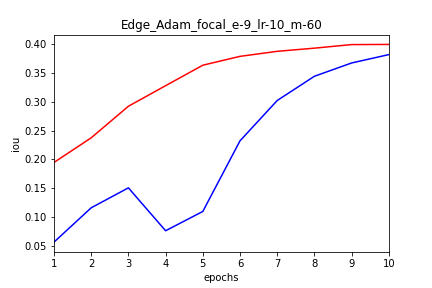
\includegraphics[width=\textwidth]{imgs/lambda/5/Edge_Adam_focal_e-9_lr-10_m-60_13_May_2022-22:32.png}
        \caption{Edge.}
    \end{subfigure}
    \caption{Lambda: 0.05}
\end{figure}

\begin{figure}[H]
    \centering
    \begin{subfigure}[b]{0.45\textwidth}
        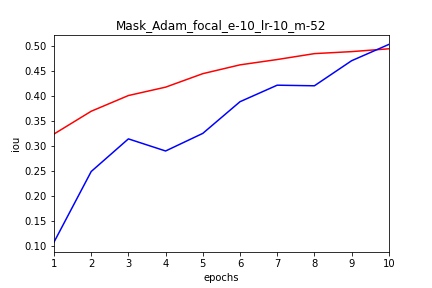
\includegraphics[width=\textwidth]{imgs/lambda/9/Mask_Adam_focal_e-10_lr-10_m-52_13_May_2022-22:50.png}
        \caption{Mask.}
    \end{subfigure}
    \hfill
    \begin{subfigure}[b]{0.45\textwidth}
        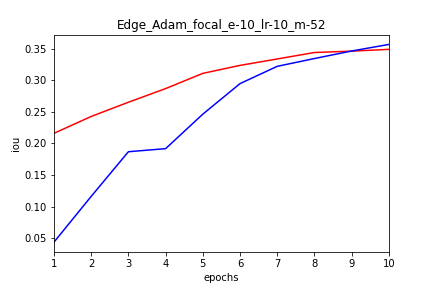
\includegraphics[width=\textwidth]{imgs/lambda/9/Edge_Adam_focal_e-10_lr-10_m-52_13_May_2022-22:50.png}
        \caption{Edge.}
    \end{subfigure}
    \caption{Lambda: 0.09}
\end{figure}
From plots we can tell that edge awarness is important for our model: stability-wise
and score-wise.
\newpage

\section{Analysis of Edge Correlations}
In my best runs edges definitely look like edges of masks and there is correlation.
Worsts happen just at the beginning of training or when model starts to overfit.
\begin{figure}[h]
    \centering
    \begin{minipage}[b]{0.45\textwidth}
        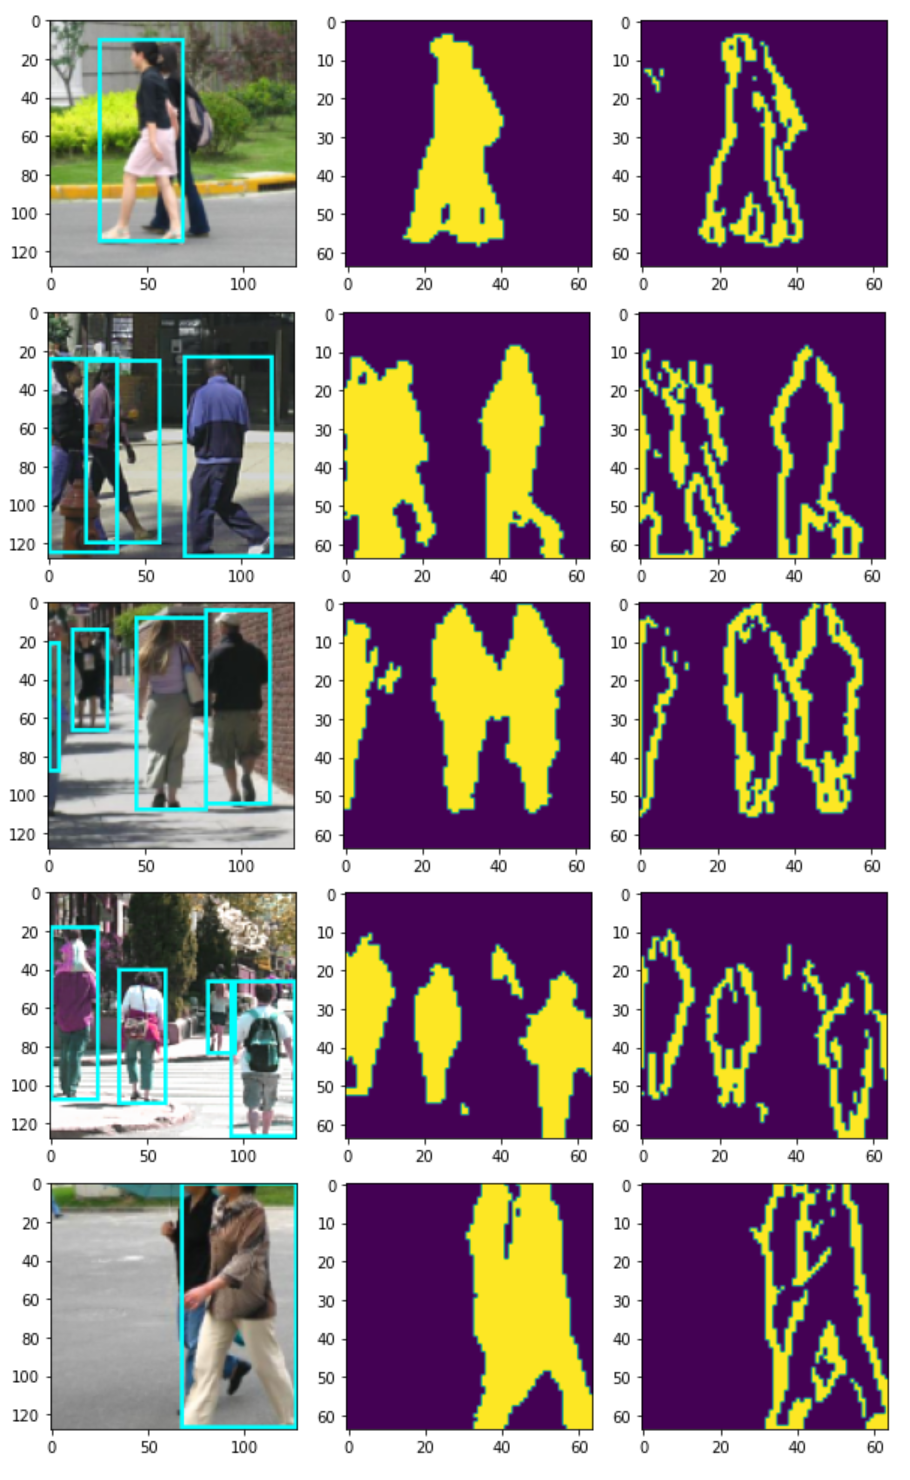
\includegraphics[width=\textwidth]{imgs/best.png}
        \caption{Good.}
    \end{minipage}
    \hfill
    \begin{minipage}[b]{0.45\textwidth}
        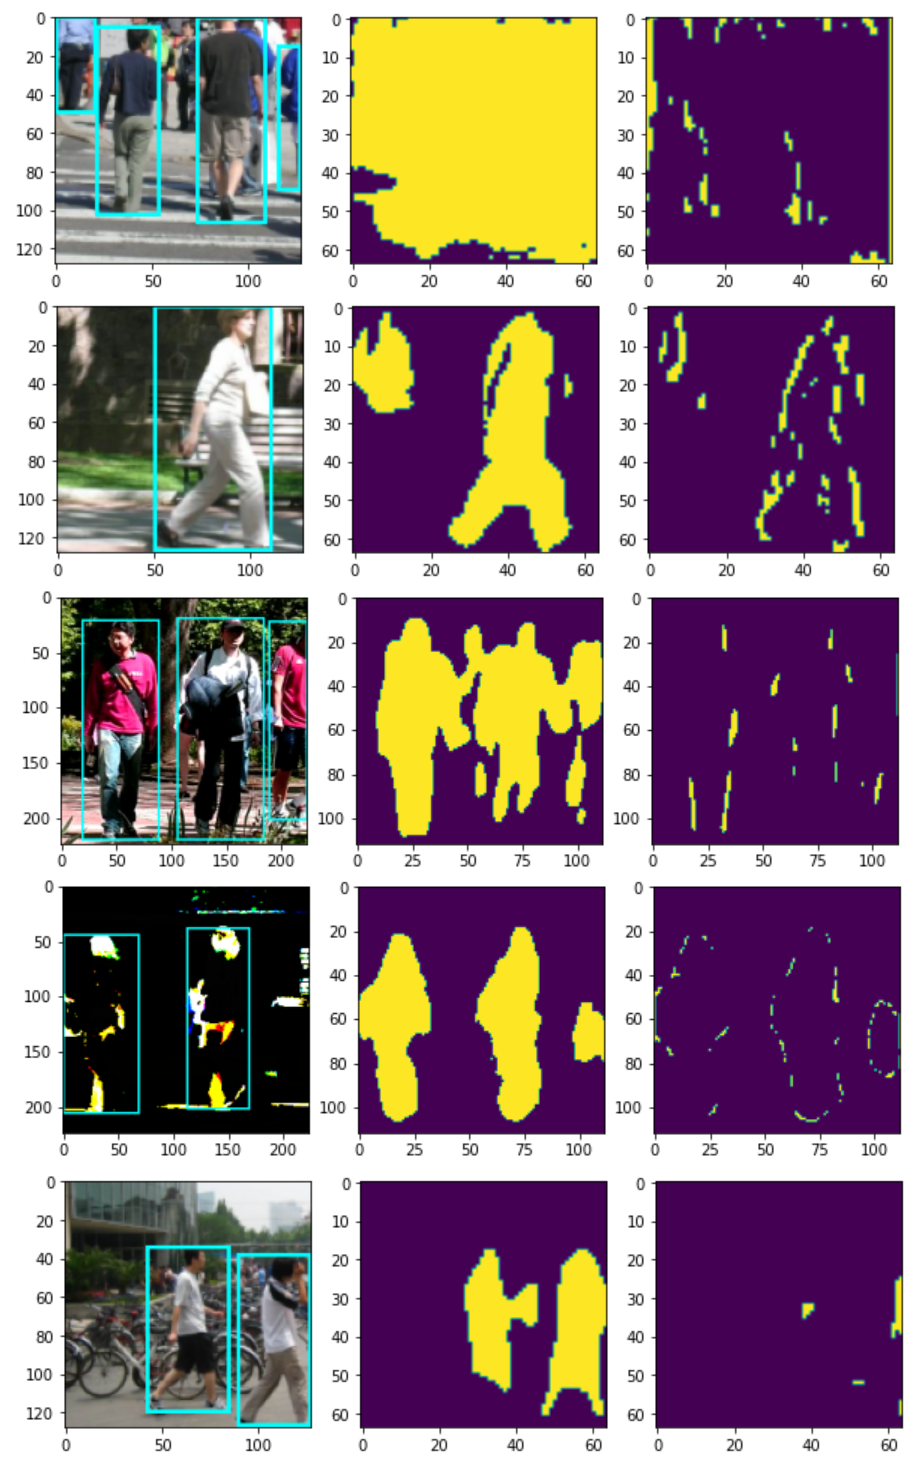
\includegraphics[width=\textwidth]{imgs/worst.png}
        \caption{Bad.}
    \end{minipage}
\end{figure}

\end{document}
